% Options for packages loaded elsewhere
\PassOptionsToPackage{unicode}{hyperref}
\PassOptionsToPackage{hyphens}{url}
%
\documentclass[
]{book}
\usepackage{amsmath,amssymb}
\usepackage{lmodern}
\usepackage{iftex}
\ifPDFTeX
  \usepackage[T1]{fontenc}
  \usepackage[utf8]{inputenc}
  \usepackage{textcomp} % provide euro and other symbols
\else % if luatex or xetex
  \usepackage{unicode-math}
  \defaultfontfeatures{Scale=MatchLowercase}
  \defaultfontfeatures[\rmfamily]{Ligatures=TeX,Scale=1}
\fi
% Use upquote if available, for straight quotes in verbatim environments
\IfFileExists{upquote.sty}{\usepackage{upquote}}{}
\IfFileExists{microtype.sty}{% use microtype if available
  \usepackage[]{microtype}
  \UseMicrotypeSet[protrusion]{basicmath} % disable protrusion for tt fonts
}{}
\makeatletter
\@ifundefined{KOMAClassName}{% if non-KOMA class
  \IfFileExists{parskip.sty}{%
    \usepackage{parskip}
  }{% else
    \setlength{\parindent}{0pt}
    \setlength{\parskip}{6pt plus 2pt minus 1pt}}
}{% if KOMA class
  \KOMAoptions{parskip=half}}
\makeatother
\usepackage{xcolor}
\IfFileExists{xurl.sty}{\usepackage{xurl}}{} % add URL line breaks if available
\IfFileExists{bookmark.sty}{\usepackage{bookmark}}{\usepackage{hyperref}}
\hypersetup{
  pdftitle={PHP For The Web: Enough to be Dangerous},
  pdfauthor={Bryan Hoffman},
  hidelinks,
  pdfcreator={LaTeX via pandoc}}
\urlstyle{same} % disable monospaced font for URLs
\usepackage{longtable,booktabs,array}
\usepackage{calc} % for calculating minipage widths
% Correct order of tables after \paragraph or \subparagraph
\usepackage{etoolbox}
\makeatletter
\patchcmd\longtable{\par}{\if@noskipsec\mbox{}\fi\par}{}{}
\makeatother
% Allow footnotes in longtable head/foot
\IfFileExists{footnotehyper.sty}{\usepackage{footnotehyper}}{\usepackage{footnote}}
\makesavenoteenv{longtable}
\usepackage{graphicx}
\makeatletter
\def\maxwidth{\ifdim\Gin@nat@width>\linewidth\linewidth\else\Gin@nat@width\fi}
\def\maxheight{\ifdim\Gin@nat@height>\textheight\textheight\else\Gin@nat@height\fi}
\makeatother
% Scale images if necessary, so that they will not overflow the page
% margins by default, and it is still possible to overwrite the defaults
% using explicit options in \includegraphics[width, height, ...]{}
\setkeys{Gin}{width=\maxwidth,height=\maxheight,keepaspectratio}
% Set default figure placement to htbp
\makeatletter
\def\fps@figure{htbp}
\makeatother
\setlength{\emergencystretch}{3em} % prevent overfull lines
\providecommand{\tightlist}{%
  \setlength{\itemsep}{0pt}\setlength{\parskip}{0pt}}
\setcounter{secnumdepth}{5}
\usepackage{booktabs}
\usepackage{amsthm}
\makeatletter
\def\thm@space@setup{%
  \thm@preskip=8pt plus 2pt minus 4pt
  \thm@postskip=\thm@preskip
}
\makeatother
\ifLuaTeX
  \usepackage{selnolig}  % disable illegal ligatures
\fi
\usepackage[]{natbib}
\bibliographystyle{apalike}

\title{PHP For The Web: Enough to be Dangerous}
\author{Bryan Hoffman}
\date{2022}

\begin{document}
\maketitle

{
\setcounter{tocdepth}{1}
\tableofcontents
}
\hypertarget{introduction-and-prerequisites}{%
\chapter{Introduction and Prerequisites}\label{introduction-and-prerequisites}}

Howdy!

This is going to be a very brief but hopefully very helpful text for beginners. I chose PHP because it is a great language to get up and running with. WordPress and Laravel are great options for the web, and PHP is a robust language on its own.

Don't just read along. Try things out. Never copy and paste the example code. Write it yourself and make it your own. I'll try to provide helpful loose ends for you to jump into if you feel inspired. I'll try to make my examples varied and show different possible applications. Math is inevitable. Sorry. This is a gentle text that requires very little prior knowledge of mathematics. In other words: you definitely don't need calculus for this text. This text is written to gradually introduce programming concepts as scaffolding before exploring more complex examples.

I encourage you to use the terminal. If you're running Windows, I would suggest setting up the Windows Linux Subsystem. If you're running Mac OS, you've already got a terminal. Linux is my preference, but you can jump into this material from any OS.

Commands for the terminal will have a ``\textgreater{}'' character at the beginning. If you're unfamiliar with using the terminal, you'll find some helpful commands to get started below.

\textgreater ls : list all the documents in your current directory

\textgreater cd : change directory

\textgreater php -a : start an interactive PHP shell

\textgreater man : retrieve a manual for using a command

It is customary to suggest that you start by reading the manual on the manual command. You can do this by running \textgreater man man in your terminal.

\hypertarget{printing}{%
\chapter{Printing in the Terminal and on the Web}\label{printing}}

Let's write some code!

Open a text editor of your choice to get started. You'll be saving files with a ``.php'' extension. To begin you'll write:

\begin{verbatim}
<?php
\end{verbatim}

This signifies that there's php code after it. If you don't include this, things won't work.

To create a variable in PHP, you need to use the dollar sign. PHP isn't the only language to do this, for example, Perl also prefaces variable names with a special character. Let's \textbf{declare} a variable.

\begin{verbatim}
<?php 

$variable;
\end{verbatim}

Now let's \textbf{initialize} the same variable:

\begin{verbatim}
<?php

$variable;

$variable = "string";
\end{verbatim}

One can combine these steps. If we declare and initialize \$variable on the same line, our full code will now look something like:

\begin{verbatim}
<?php

$variable = "string";
\end{verbatim}

Save your file as example\_0.php or something like that. Then in your terminal, type:

\textgreater php example\_0.php

Absolutely nothing should happen, but there shouldn't be any errors. It is a working piece of code, but we've not told it to display anything. Let's get it to display to the terminal by adding some more code. We need to add a print statement. Modify your file so it matches this:

\begin{verbatim}
<?php

$variable = "string";

print("The value of \$variable is: ".$variable."\n");
\end{verbatim}

There's a lot going on here. The first thing to note is that the period ``.'' is like a plus sign for strings. Gluing strings together is called \textbf{concatenation}. The backslash ``\textbackslash{}'' before the first instance of \$variable is called an \textbf{escape character}. Without it, the program would print ``The value of string is: string'' not ``The value of \$variable is: string'' and I wanted to have it print ``\$variable'' literally. Using single quotes would have worked as well but if I had ran:

\begin{verbatim}
<?php

$variable = "string";

print('The value of $variable is: '.$variable.'\n');
\end{verbatim}

The ``\textbackslash n'' in single quotes would've come out as ``\textbackslash n'' literally, and I didn't want that. I included the ``\textbackslash n'' to print a new line. In the terminal, this will make things look a lot nicer.

You can very easily print to the web instead and with no modifications to the code that's already writing to the terminal. Instead of running it with the command:

\textgreater php example\_0.php

Run:

\textgreater php -S localhost:8080 example\_0.php

and using a browser of your choice, navigate to: \url{http://localhost:8080/} and you'll see the message printed in the browser instead of the terminal. How easy was that!?

\hypertarget{branching}{%
\chapter{Branching and Conditionals}\label{branching}}

Let's open up our text editor and create a new file starting with ``\textless?php'' and save it to a file with a name like branching\_example.php or similar.

PHP has some \textbf{operators}, and only a few will be intuitive. When doing math, ``+'', ``-'', ``*``, and''/'' probably behave like you'd guess. There's an operator ``\%'' called ``modulo'' that is really useful. If you remember remainders, the modulo operator will result in the remainder after division. For example, 7\%3 is 1, because 3 goes into 7 twice with 1 as the remainder. 17\%4 is also 1, and that's because 4 goes into 17 four times with 1 as the remainder. Let's say you have a variable \$my\_value and you want to see if it's even or odd. Another way to phrase this is: ``does the number have a remainder when divided by 2?'' and if the answer is ``yes,'' that means it's odd, and if the answer is ``no,'' that means the number is even. Let's turn this into code:

\begin{verbatim}
<?php

$my_value = 1; // is it odd or even?

if($my_value%2 != 0 ) { // the number has a remainder when divided by two
    print("It is odd!\n");
}
if($my_value%2 == 0 ) { // the number has no remainder when divided by two
    print("It is even!\n");
}
\end{verbatim}

The first thing to note is the double slashes ``//'' which indicate a comment. You can write comments to clarify things for yourself and others who read your code. If you want to make a multi-line comment, use ``/*'' and ``*/'' instead of ``//'' like this:

\begin{verbatim}
<?php 

/*
 * Here is a line
 * Here's another
 * Wow a third line, and it's still a single comment?
 */
\end{verbatim}

You can put asterisks on all the lines of your comment and line them up vertically to make it look better. Some text editors will do this formatting by default, but formatting it like that is not necessary. The ``/*'' and ``*/'' parts are all that's necessary to comment out multiple lines. This is a nice \textbf{debugging} technique.

The second part to note is the if-statement. This lets us check if something is true and do something if it is. Here's another example:

\begin{verbatim}
<?php

$this_variable_is_false = false;

if($this_variable_is_false = true) {
    print("Will this run?\n")
}
\end{verbatim}

So, what do you think? Will that print statement run? Test it out for yourself.

The result might surprise you, but let me explain. In the previous example, the expression inside the if-statement's parentheses used a single equals sign ``='' and we've seen that a single equals sign is what you use to assign a value to a variable. The program understands it this way, and will assign true to the variable and then the value is true and the part of the if statement inside the curly braces ``\{ \}'' is executed. To actually check if the variable is true, we use a different operator than ``='' because we don't want to assign a value to a variable, we want to compare a value to a variable. Instead of the single equals sign, we'll use a double equals sign ``=='' as in the first code example in this chapter. That example also used ``!='' which will return true when comparing unlike values, or in other words the values are not equal to each other. Using ``='' instead of ``=='' in if-statements is a potential mistake for beginners that's quite easy to make.

When a variable contains true or false, it's called a boolean. This name is an homage to a mathematician, George Boole. If the part of the if-statement in the parentheses evaluates to true, the code in the curly braces executes. Since booleans are true or false, you can write if-statements like this:

\begin{verbatim}
<?php 

$my_boolean = true;

if($my_boolean) {
    print("\$my_boolean is true!\n");
}
\end{verbatim}

There are more operators. In the way that ``+'' and ``-'' are for adding and subtracting numbers, there are other sorts of operators for doing mathematics with booleans and other data types. Is false plus false, false? According to PHP, false + false is 0. There's better ways to work with booleans, than ``+'' and ``-'' so let's use them! I'm pleased to introduce ``\&\&'' and ``\textbar\textbar{}'' which can be read as ``and'' and ``or'' respectively. And now an example with these operators in use:

\begin{verbatim}
<?php 

if(true && true) {
    // code here will run
}

if(true && false) {
    // code here won't run
}

if(true || true) {
    // code here will run
}

if(true || false) {
    // code here will run
}
\end{verbatim}

An if-statement can contain another if-statement, like so:

\begin{verbatim}
<?php 

$my_integer = -27;
$my_boolean = true;

if($my_integer < 0) {
    if($my_boolean) {
        // do something
    } 
}
\end{verbatim}

An if-statement within another if-statement can be called a \textbf{nested} if-statement. In some cases, you might want to use an else-statement. A simple if-statement is like saying ``do this under this circumstance'' whereas an if-else statement is like ``do this under this circumstance, otherwise do that instead.''

Sometimes, when I'm grocery shopping, I act like a program. To me, there's nothing like an avocado. I like avocados, and there's no replacement in my mind suitable for them\ldots{} but they're usually pricey. If they're too pricey, I just don't get them. But with fruit, I like berries more than apples, but berries are usually pretty expensive. If berries are on sale, I'll get berries, otherwise I'll just get apples. Here's how that would look as some PHP code:

\begin{verbatim}
<?php

if($current_avocado_price < $my_max_avocado_price) {
    // buy some avocados
}

if($blueberries_on_sale) {
    // buy some berries
} else {
    // buy some apples
}
\end{verbatim}

Let's start tackling a somewhat common interview challenge. Fizzbuzz is a very simple game that works for any number of players. Someone begins counting at 1, the next person increments the number and says the number unless the number is divisible by three or five. If it's divisible by three, say fizz, if it's divisible by five, say buzz, if it is divisible by both, say fizzbuzz. Here's some PHP code that takes a number and prints the appropriate response as if it were playing fizzbuzz:

\begin{verbatim}
<?php


//the number we want to test
$number_to_test = 25;

// initialize to false by default before testing
$divisible_by_three = false;
$divisible_by_five = false;

if($number_to_test % 3 == 0) {
    $divisible_by_three = true;
}

if($number_to_test % 5 == 0) {
    $divisible_by_five = true;
}

if($divisible_by_three && $divisible_by_five) {
    print("fizzbuzz\n");
}

if($divisible_by_three == true && $divisible_by_five == false) {
    print("fizz\n");
}

if($divisible_by_three == false && $divisible_by_five == true) {
    print("buzz\n");
}

if($divisible_by_three == false && $divisible_by_five == false) {
    print($number_to_test."\n");
}
\end{verbatim}

Exercises:

\begin{enumerate}
\def\labelenumi{\arabic{enumi}.}
\item
  Modify the fizzbuzz example to use if-else statements or nested if-statements. Check your edited version for correctness by trying various values (3, 17, 45, 61, \&c.) and checking the output for correctness (fizz, 17, fizzbuzz, 61, \&c.). As it's currently written, all six if-statements are checked everytime the program is run. You can make the program more efficient by using if-else-statements and nested if-statements and reducing how many conditions need to be checked. Thinking about efficiency won't really matter a whole lot here, but if you are one day running a program billions of times, making it run in half the time could save lots of time and money. Unlike math, correctness isn't enough. Programming challenges can often be solved in multiple ways that are equally correct. Two methods might be correct, but one might be better because it runs in less time or uses less resources.
\item
  Using if-statements and the modulo operator, can you write a program that can tell you if a whole number from 1 to 100 is a prime number?
\end{enumerate}

\hypertarget{loops}{%
\chapter{Loops}\label{loops}}

Before we get into this section of the text, you need to know how to interrupt the terminal. If a program is running, and you want to exit it, press Ctrl+C, just like you were copying some text. It is possible to write programs that never end. The next code sample is one such program. Save the following code into a file and run it. You'll need to interrupt the program, otherwise it'll execute forever! Press Ctrl+C once you've had enough.

\begin{verbatim}
<?php

while(true) {
    print("A");
}
\end{verbatim}

While-loops have a close relative, the for-loop. The while-loop is very similar to an if-statement. It executes the code in the curly braces when the condition in the parentheses is true. The key difference between an if-statement and a while-loop is that when the program reaches the closing curly brace ``\}'' of a while-loop, it hops back to the top and checks the condition again. This can repeat indefinitely as the prior example demonstrated.

A for-loop looks like this:

\begin{verbatim}
for($i = 0; i < $max_value; $i++) {
    // do stuff
}
\end{verbatim}

This text will begin omitting ``\textless?php'' unless it's a full file's contents that is being displayed.

Let's break the for-loop down. In the parentheses, we declare and initialize a variable, then comes a conditional, and the last part is a piece of code that gets run with every loop. In the last part, we are simply incrementing and storing the value, so ``\$i = \$i + 1'' would have the same effect as ``\$++'' here. If the conditional part evaluates to false, the for-loop stops.

Sometimes, a certain task feels like a job for a for-loop, and other tasks feel like they'd be best implemented with a while-loop.

Just like if-statements, loops can be nested. Here's an example of a nested for-loop that will print a rectangle of asterisks with the dimensions held in the variables \$width and \$height:

\begin{verbatim}
$width = 10;
$height = 10;

for($i = 0; $i < $height; $i++) {
    for($j = 0; $j < $width; $j++) {
        print("*");
    }
    print("\n");
}
\end{verbatim}

Exercises:

\begin{enumerate}
\def\labelenumi{\arabic{enumi}.}
\item
  Modify the fizzbuzz program from the last chapter to use a loop. Have it run from 1 until a maximum value you can set by editing the value of a variable.
\item
  Use a nested for-loop to print a multiplication table. Try to format it well. Note the symmetry of it. Since 4*8 is equal to 8*4, are we making the computer do more work than it needs to?
\item
  Can you modify the code that prints a rectangle full of asterisks so that it prints a box instead? With \$height = 4 and \$width = 5, your code should output:
\end{enumerate}

\begin{verbatim}
*****
*   *
*   *
*****
\end{verbatim}

\hypertarget{functions-and-recursion}{%
\chapter{Functions and Recursion}\label{functions-and-recursion}}

A function is a unit of code. You can write a piece of code in a function and give it a name and then use it again and again from different places. It's wise to create your own functions as your projects get more complex. There are many functions available to you out of the box. We're going to use one such function ``rand()'' -- a random number generator -- to calculate pi using a technique called the Monte Carlo method. Now, of course, getting the value of pi isn't hard. With PHP,
we could make use of a special variable ``M\_PI'' that you'll notice lacks the ``\$'' which most php variables begin with. It'll be fun to use the Monte Carlo method, and we'll compare our value to M\_PI to gauge how accurate our method is.

In your terminal, run \textgreater php -a to get access to an interactive shell. I find this useful for trying out snippets of code. Try it yourself. If we simply use rand() we get a bunch of large positive numbers. You can run this multiple times in an interactive session to see what it outputs.

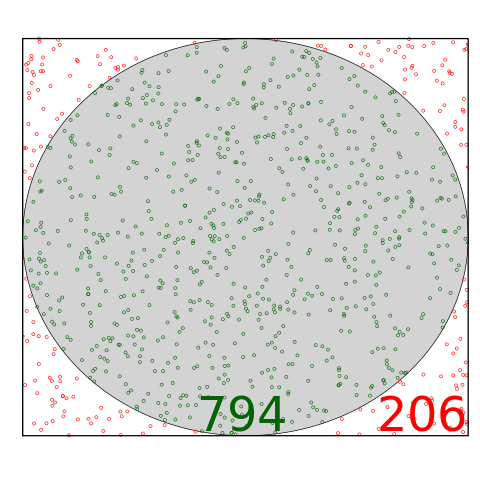
\includegraphics{480px-Circle_area_Monte_Carlo_integration2.svg.png}

To calculate pi, I want to generate two numbers to make a coordinate. The range of each random number should be from -1 to 1. We'll check the coordinate and see if it is inside a circle with radius one. After enough random points are placed, we can tease pi out of the ratio of total points and points inside the circle.

\begin{verbatim}
<?php

$x=0;
$y=0;
$inside_total = 0;
$total = 0;

for($i = 0; $i < 10000; $i++) {
    // generate random numbers in (-10000,10000) and scale to (-1, 1)
    $x = rand(-10000,10000)/10000;
    $y = rand(-10000,10000)/10000;
    // check if the random point is inside the circle
    if($x*$x+$y*$y <= 1 ) {
        // keep track of points inside the circle
        $inside_total++;
    }
    // keep track of all points
    $total++;
}
// estimate pi
$pi_approx = 4*($inside_total/$total);
// calculate error
$error=(($pi_approx-M_PI)/M_PI)*100;
print("Pi is approximately: $pi_approx\n");
print("The error was: ".$error."%\n");
\end{verbatim}

Let's write our own function now. We'll continue with something similar to what we did in the Monte Carlo example. Let's code a function that takes a coordinate and a radius, and returns true if the coordinate is inside a circle of the specified radius and false otherwise. A function like that looks like this:

\begin{verbatim}
function inside_circle ($x, $y, $radius) {
    if($x*$x+$y*$y <= $radius**2) { // "$a**$b" is $a raised to the power $b
        return true;
    } else {
        return false;
    }
}
\end{verbatim}

We use return to pass a result back to wherever the original \textbf{call} to the function came from. We can now combine our last two pieces of code into this:

\begin{verbatim}
<?php

$x=0;
$y=0;
$inside_total = 0;
$total = 0;

// functions need to be declared before they are used
function inside_circle ($x, $y, $radius) {
    if($x*$x+$y*$y <= $radius**2) { // "$a**$b" is $a raised to the power $b
        return true;
    } else {
        return false;
    }
}

for($i = 0; $i < 10000; $i++) {
    // generate random numbers in (-10000,10000) and scale to (-1, 1)
    $x = rand(-10000,10000)/10000;
    $y = rand(-10000,10000)/10000;
    // check if the random point is inside the circle and
    // replace the conditional with a call to inside_circle
    if(inside_circle($x, $y, 1)) { 
        // keep track of points inside the circle
        $inside_total++;
    }
    // keep track of all points
    $total++;
}
// estimate pi
$pi_approx = 4*($inside_total/$total);
// calculate error
$error=(($pi_approx-M_PI)/M_PI)*100;
print("Pi is approximately: $pi_approx\n");
print("The error was: ".$error."%\n");
\end{verbatim}

If-statements can contain if-statements, loops can contain loops, and functions can contain functions! But functions can do something a bit spooky, a function can call itself from inside itself. This is called \textbf{recursion}. Let's write a recursive function to find the n-th value in the Fibonacci sequence. The Fibonacci sequence begins 1, 1, 2, 3, 5, 8, \ldots{} and the rule for generating the next term is to add the last two.

\begin{verbatim}
function fib($n) {
    if($n == 1 || $n == 2) {
        return 1;
    } else {
        return(fib($n-1)+fib($n-2));
    }
}
\end{verbatim}

I'll encourage you to try out the interactive PHP shell once more. Start it by entering \textgreater php -a in your terminal. Write the fib() function yourself and then you can call it and print the results you get by typing \textgreater echo fib(1);

``echo'' is just another way to print things in PHP. If you didn't include ``echo'' you wouldn't see anything. Calling fib() just returns a value, but doesn't do anything with it. Most of the time, you'll do something with it like store it in a variable or print it.

Exercises:

\begin{enumerate}
\def\labelenumi{\arabic{enumi}.}
\item
  Write a recursive function to calculate the factorial of a positive integer or zero. It might be helpful to know that 0! is equal to 1.
\item
  Can you modify the code utilizing the Monte Carlo method to calculate pi, and run the simulation in three dimensions or even higher dimensional spaces? Does changing the dimension of the simulation have any impact on the accuracy of the result?
\end{enumerate}

\hypertarget{GET}{%
\chapter{HTTP GET Variables}\label{GET}}

There is something called the Collatz Conjecture. It's not known whether it is true or false. Start with any positive integer. If it's odd, you multiply it by 3 and add 1 to it. If it's even, you divide it by two. Keep doing this and the Collatz Conjecture claims you'll always eventually arrive at 1. Let's see this in action with 5.

5 is odd. 3*5+1 = 16. 16 is even. 16/2 = 8. 8 is even. 8/2 = 4. 4 is even. 4/2 = 2. 2 is even. 2/2 = 1.

So, 5 was not a counter example. Let's code the logic of the Collatz Conjecture before we connect to the web. Our first bit of code:

\begin{verbatim}
<?php

$value = 17;

while($value!=1) {
    if($value%2==1) {
        // echo the first part of the statement
        echo "$value is odd. 3*$value+1 = ";
        // actually change $value to the new value
        $value=3*$value+1;
        // echo the last part with $value update
        echo "$value\n";
    }
    else {
        // echo the first part of the statement
        echo "$value is even. $value/2 = ";
        // actually change $value to the new value
        $value=$value/2;
        // echo the last part with $value update
        echo "$value\n";
    }
}
\end{verbatim}

Run it a few times in the console with different values. Everything I've tried has gone to 1 after some number of steps. Once you've gotten a sense of things, let's connect to the web. Instead of ``\$value = 17;'' we're going to replace the code on line 3 with this:

\begin{verbatim}
if(isset($_GET["value"])) {
    $value = $_GET["value"];
} else {
    $value = rand(1,100);
}
\end{verbatim}

Name your file something like collatz.php and serve it by typing the following in your terminal:

\textgreater php -S localhost:8080 collatz.php

In your web browser, head to \url{http://localhost:8080} and give it whirl. I've set it up so it will generate a random positive integer if one isn't provided. Things might be looking pretty messy. For web, instead of ``\textbackslash n'' we'll want to use ``'' the HTML element for break. Replace instances of ``\textbackslash n'' with ``'' and refresh your browser. You'll end up with a different looking page every time you refresh because it is dynamically generated. Refresh it once more and based on a new random integer, you'll see another entirely different page.

We can actually input a number now. In your browser, if you go to the url: \url{http://localhost:8080?value=81} it will run for the value you provided through the URL. Give that a try now. Since we're utilizing the web now, let's take advantage. Let's put a couple lines of code between the if-else-statement handling the \$\_GET variable and the start of the while-loop. Something like:

\begin{verbatim}
echo '<a href="/?value='.($value+1).'">Try '.($value+1).'</a> | ';
echo "<a href=\"/\">Try another random integer</a><br>";
\end{verbatim}

Writing combined HTML and PHP like this can be really confusing. You know how ``\textless?php'' needs to be at the beginning of our PHP files for a file to execute properly? Now is a good time to show another way to write PHP and HTML together. Take a look at this example file:

\begin{verbatim}
<?php

$value_0 = true;
$value_foo = "bar";

// we can close the php tag with and just write plain HTML for a bit
?>

<h1>Heading 1</h1>
<p>This is a paragraph.</p>

<?php 

// we can begin an if-statement in one PHP block ...

if($value_0) { 

?>

The value of $value_foo is: <?php echo $value_foo; ?></p>

<?php 

// ... and end it in another

} 

?>
\end{verbatim}

Exercises:

\begin{enumerate}
\def\labelenumi{\arabic{enumi}.}
\item
  What happens if you put a very large integer into the Collatz Conjecture example? What happens if you put in a negative integer? What happens if you put in something like ``potato''? When writing ``real-life'' applications, at best, you'll get bad input from users, and at worst, hackers will attempt to maliciously exploit holes in your application. Can you think of ways you could already improve this example web application?
\item
  Try to create a multi-lingual site where the language can be passed in as a URL parameter. For example: localhost:8080/?lang=es might load in Spanish, and available languages might be shown as flags that can be clicked.
\item
  Try and write a choose your own adventure story that works in the browser. You can use page numbers in the URL, or get creative with things like localhost:8080/?you\_are=running\_away\_from\_a\_troll
\end{enumerate}

\hypertarget{Forms-and-Files}{%
\chapter{Forms and Files}\label{Forms-and-Files}}

I've got a vision of what to build next. Let's try to build a very simple editable blog. In ``real world'' applications, we'd probably make use of databases, but for our purposes, let's build the thing by writing to files. By writing to file, we can make things \textbf{persistent}. Storing things in PHP variables only lasts as long as the program is running, but saving results of programs to files or a database can leave a record. A record is something we can pull up again and again, and modify and save. For a lot of applications, persistent data is a necessity.

Let's start by creating a simple HTML file at index.html:

\begin{verbatim}
<html>
  <body>
    <h1>Welcome to My Personal Homepage</h1>
    <p>I can neither confirm nor deny ...</p>
    <p>PHP may or may not mean Personal HomePage</p>
  </body>
</html>
\end{verbatim}

Displaying this with PHP is rather straight-forward. We create a file at index.php at put the following in it:

\begin{verbatim}
<?php

require('index.html');
\end{verbatim}

Serve your webpage with the following command in your terminal \textgreater php -S localhost:8080 index.php and navigate to it with your browser. You'll see index.html rendered. PHP has pulled index.html in and rendered it in the browser all as a result of including that single ``require(`index.html');'' line.

We want to be able to edit index.html from the browser. Let's include a link, but not in index.html. We'll put the link in index.php, so that we can click to get into an editing mode. Include:

\begin{verbatim}
<a href="/?edit=true">Edit</a>
\end{verbatim}

in your index.php file. You can use ``?\textgreater{}'' to exit the PHP code block and put it in as plain HTML or if you want the challenge, try to echo or print it with PHP.

In edit mode, we shouldn't render the HTML file, we should pull it into a text field that can be edited and saved. We'll use ``isset()'' to check the ``\$\_GET'' \textbf{super global} variable, and if we see ``\$\_GET{[}`edit'{]}'' exists, we'll render this form instead. To do that, we need to pull the file in to our program in a slightly different way. Below is the full code of index.php with these additions made:

\begin{verbatim}
<?php

// If the form was submitted write changes to file
if(!empty($_POST["text"])) {
    // file_put_contentes writes to file
    file_put_contents('index.html',$_POST["text"]);
}

if(isset($_GET['edit'])) {
    // file_get_contents reads from file
    $file_contents = file_get_contents('index.html');
    // echo our form elements with $file_contents in the textarea
    echo '<form method="post" action="index.php">';
    echo '<textarea id="text" name="text">';
    echo $file_contents;
    echo '</textarea>';
    echo '<input type="submit" value="submit">';
    echo '</form>';
} else {
    // render index.html
    require('index.html');
    // link to access edit mode
    echo '<a href="/?edit=true">Edit</a>';
}
\end{verbatim}

That ``\$\_POST{[}{]}'' variable works much like ``\$\_GET{[}{]}'' does. It exists because we submitted a form or something similar, but if we simply load and render a page, nothing would be in the variable. By checking the contents of the variable before doing anything else, we can intercept the form data and save it to file before rendering the page. If we had reversed the order, the experience in the browser would be strange.

Order is important in programming. The math term for things that are order dependent is non-abelian. If you walk east for a mile and then walk north a mile, the result would be the same even if you switched the order. You'd end up in the same place, a little over 1.4 miles northeast of where you started. If you display a file and then make changes to it, well, that's not going to have the same results as making the changes to it and then displaying it.

You've now built a very simple blog! Have fun and make it your own!

Exercises:

\begin{enumerate}
\def\labelenumi{\arabic{enumi}.}
\tightlist
\item
  Can you build a web application that functions as a diary? Instead of opening a file and editing it, you might want to append to the file so that previous contents doesn't get overwritten.
\end{enumerate}

\hypertarget{SESSION}{%
\chapter{SESSION}\label{SESSION}}

We don't want just anyone to be able to come along and edit our blog. Let's make an effort to protect it. In this effort, we will encounter another super global ``\$\_SESSION{[}{]}'' along the way. We'll be pretending this is secure. In ``real world'' applications, it's best to go with an established method and not reinvent the wheel yourself. But, for us right now, reinventing the wheel might prove to be an enlightening experience!

So, what's this ``\$\_SESSION'' super global do? It holds information about the user and their session with the server. This is where you might find a username or perhaps time zone details and other personal settings.

We'll create a session in one line at the top of index.php and then store ``true'' in ``\$\_SESSION{[}`authenticated'{]}'' when the client proves they know a secret pin. We should take care to hide the ``edit mode'' from users who aren't logged-in. For a user who wants to log in, navigating to edit mode will prompt them for the pin. It's not the best security method, but this method of security by obscurity does work. Keep the sensitive details out of sight. Why advertise your log in
portal with a link from your navigation bar? Users who are in the know, will know to navigate to the log in page, no need to post it publicly!

Here's our updated code:

\begin{verbatim}
<?php

// start a session
session_start();

// super secret not very secure pin
$secret_pin = "123456";

// Check if the secret pin form was submitted
if(!empty($_POST["pin"])) {
    // check pin for correctness
    if($_POST["pin"] == $secret_pin){
        // set clients status to authenticated
        $_SESSION['authenticated'] = true;
    }
}

// If the form was submitted write changes to file
if(!empty($_POST["text"])) {
    // file_put_contentes writes to file
    file_put_contents('index.html',$_POST["text"]);
}

if(isset($_GET['edit'])) {
    // check for auth
    if(isset($_SESSION['authenticated'])) {
        // file_get_contents reads from file
        $file_contents = file_get_contents('index.html');
        // echo our form elements with $file_contents in the textarea
        echo '<form method="post" action="index.php">';
        echo '<textarea id="text" name="text">';
        echo $file_contents;
        echo '</textarea>';
        echo '<input type="submit" value="submit">';
        echo '</form>';
    } else {
        // if not authenticated
        // echo our form elements with $file_contents in the textarea
        echo '<form method="post" action="index.php">';
        echo '<input type="text" name="pin">';
        echo '<input type="submit" value="submit">';
        echo '</form>';
    }
} else {
    // render index.html
    require('index.html');
    // link to access edit mode only show to authenticated users
    if(isset($_SESSION['authenticated'])) {
        echo '<a href="/?edit=true">Edit</a>';
    }
}
\end{verbatim}

Serve your web application by running: \textgreater php -S localhost:8080 index.php

Navigate to \url{http://localhost:8080?edit} to log in. That's it! We've somewhat secured the simple blog we made in the last chapter. By no means is this secure-secure, but it is at least better than nothing!

Exercises:

\begin{enumerate}
\def\labelenumi{\arabic{enumi}.}
\item
  A PHP file might be revealed by the browser in certain circumstances. For example, forget an opening ``\textless?php'' and a chunk of code might show up in the browser. To prevent this from ever happening with ``\$secret\_pin'', try to isolate that code in another file and load it into index.php instead.
\item
  Imagine you shared this simple blog with a friend and they were making edits at the same time as you. What kind of errors could happen as a result? How might you prevent those errors?
\end{enumerate}

\hypertarget{Next}{%
\chapter{What Next?}\label{Next}}

I'm glad you've followed along and I hope you enjoyed this brief text. In parting, I want to make an effort to direct you toward worthwhile resources and helpful philosophies.

Writing code is one thing. Writing good code is another thing entirely. I've heard of developers being gauged by their line counts per week. In one instance, the story goes, a senior developer was appalled by the move and spent the first week \textbf{refactoring} existing code. The story goes on, he solved all the bugs while making a contribution of negative lines of code. The code base was smaller after he improved it, not bigger.

Programming, writing code, developing software, whatever you want to call it, may someday be like literacy is today. There was a day when almost no one could read and write. Now a lot of people can. The same drastic change may happen with computer literacy in the future.

Computer science can be called a field in its own right, but it's the overlap of computer science and other fields that excites me the most. This is a tool that can make tools! If you pursue a totally unrelated field, you'll probably find ways to use your computer skills.

A book like this is written to stay relevant for years. Some texts will be relevant for decades and some for centuries and even millenia. Knowledge of algorithms and mathematics will future-proof you. There's a balance to things. If you only focused on mathematics, well you probably wouldn't be reading this introductory programming text! Diversify your portfolio! Make it a habit to get out of your technical comfort zone and explore new technologies every once in a while.

By the way, you don't have to pick a programming language. Read a Python book too! Sometimes Python has a tool out of the box that makes it a better choice to use.

You'll hear talk of not reinventing the wheel, or not repeating yourself. Building something from scratch can be enlightening. The key is in having discretion. Use the appropriate tools for serious applications, but try to make your own for the sake of fun and learning too.

When you have a problem, someone else may have already solved it and provided code that solves the problem. You can review their code to understand the solution, or just use their solution. Either way, you're probably better off being able to take a peek and understand a bit about the code that you run.

If you keep on this path, you might be solving problems before anybody else. Give back to the community and share your solutions. It'll lead to professional opportunities and you can empower people in the same way other open source contributors have empowered you.

If you spotted an error, have any questions or commentary, or you just want to say ``hi,'' I can be reached at bryanhoffman1@gmail.com

  \bibliography{book.bib,packages.bib}

\end{document}
